\documentclass{article}

\usepackage{amsmath, amssymb, amsfonts}
\usepackage{amsthm}
\usepackage{tikz}
\usepackage{thmtools}
\usepackage{graphicx}
\usepackage{setspace}
\usepackage{geometry}
\usepackage{float}
\usepackage{hyperref}
\usepackage[utf8]{inputenc}
\usepackage[english]{babel}
\usepackage{framed}
\usepackage{tcolorbox}
\usepackage{comment}
\usepackage{titlesec}
\usepackage{enumitem}
\usepackage{array}
\usepackage{multirow, bigdelim}
\usepackage{marginnote}
\usepackage{lipsum}
\usepackage{neuralnetwork}
\usepackage{subfigure}
\usepackage{slashed}

\usetikzlibrary{graphs}
\usetikzlibrary{shapes}
\usetikzlibrary{backgrounds}
\usetikzlibrary{calc}
\usetikzlibrary{patterns}
\usetikzlibrary{positioning, fit, arrows.meta}

\newenvironment{solution}{\textit{Solution}.}

\titleformat{\subsection}[block]{\normalfont\Large\bfseries}{\thesubsection}{1em}{}
\titleformat{\subsubsection}[hang]{\normalfont\bfseries}{}{1em}{}

%%% Problem Numbering and Formatting

\newtheorem{problem}{Problem}
\setcounter{problem}{39} % <----- IMPORTANT:  CHANGE THIS # TO THE LAST PROBLEM # OF THE PREVIOUS SET

\def \proofDistance {5pt}
\def \subheaderSpace {10pt}


%%% PAGE DIMENSIONS
\usepackage{geometry} % to change the page dimensions
\geometry{margin=1in} % for example, change the margins to 1 inches all round

\newcommand{\proofseparator}{\par\noindent\rule{\textwidth}{0.4pt}}
\newcommand{\caution}{\marginnote{
\includegraphics[width=2em]{caution.png}}}
\newcommand{\HRule}[1]{\rule{\linewidth}{#1}}


% Natural Numbers 
\newcommand{\N}{\ensuremath{\mathbb{N}}}

% Whole Numbers
\newcommand{\W}{\ensuremath{\mathbb{W}}}

% Integers
\newcommand{\Z}{\ensuremath{\mathbb{Z}}}

% Rational Numbers
\newcommand{\Q}{\ensuremath{\mathbb{Q}}}

% Real Numbers
\newcommand{\R}{\ensuremath{\mathbb{R}}}

% Complex Numbers
\newcommand{\C}{\ensuremath{\mathbb{C}}}

% Command for problem statement
\newcommand{\pb}[1]{
    \begin{problem}
    #1
    \end{problem}
}

% Define a command for custom proofs with separator
\newcommand{\pf}[1]{
    \vspace{\proofDistance}
    \begin{proof}
    #1
    \end{proof}
    \proofseparator
}

\newcommand{\sol}[1]{
    \vspace{\proofDistance}
    \begin{solution}
    #1
    \end{solution}
    \proofseparator
}

\newcommand{\makespace}[1]{\vspace{\subheaderSpace}}

\titleformat*{\section}{\Large\bfseries}
\titleformat*{\subsection}{\large\bfseries}

% ------------------------------------------------------------------------------

\begin{document}

% ------------------------------------------------------------------------------
% Cover Page and ToC
% ------------------------------------------------------------------------------

\title{ \normalsize \textsc{}
		\\ [2.0cm]
        \HRule{1.5pt} \\
		\LARGE \textbf{\uppercase{DISCRETE MATHEMATICS}
		\HRule{2.0pt} \\ [0.6cm] \LARGE{Writing Assignment 2} \vspace*{10\baselineskip}}
		}
\date{2nd Semester, 2024}
\author{\textbf{Authors} \\ 
		Paul Beggs, Thomas Sebring}

\maketitle
\newpage

% ------------------------------------------------------------------------------
% Introduction
% ------------------------------------------------------------------------------
\section{Overview}

    Every day, we rely on applications such as Google Maps to guide us on the fastest route between point A and point B. How does Google's routing system consistently determine the quickest path? This is recognized as the Shortest Path Problem, a fundamental challenge encountered in numerous real-world scenarios and applications. It is characterized by weighted graphs, where each edge is assigned a weight -- these weights can be considered as costs or ``travel times'' as exemplified by Google Maps.
    
    The Shortest Path Problem is not only a crucial aspect of navigation applications but is also a commonly encountered issue in various fields such as logistics, network design, and resource optimization. This paper will explore the principles of weighted graphs, delve into an algorithm that is used to solve the Shortest Path Problem. This exploration will provide us with valuable insights into the computational foundations behind optimizing routes and paths in diverse scenarios. (For demonstration purposes, we will only be using positive integers.)

% ------------------------------------------------------------------------------
% Body
% ------------------------------------------------------------------------------

\section{The Shortest Path}

        For any two points, there exists the shortest distance path between them. However, the shortest distance might not be a linear path, or line, between the two points. If two points are separated by more than one non-linear path, it might not be so easy to decide which path between the points is the shortest distance. Hence, as the name suggests, the Shortest Path Problem is finding what path between two points is the shortest possible distance.

        \subsubsection{Weighted Graphs}
        
            To determine the shortest total distance, we must identify all potential paths that can be traversed. Weighted graphs prove invaluable in this regard, as they illustrate each point and the respective paths connecting them. Each path is assigned a weight or distance value, signifying the distance between two points. By leveraging these distances, algorithms can be employed to calculate the potential distances between any two points and identify the shortest possible distance.

\section{Dijkstra's Algorithm}

    \subsection{Using Djikstra's Algorithm}

        Dijkstra's Algorithm is one of many algorithms that calculates the possible distances between any two points to find the shortest possible distance. It requires maintaining a separate list of points that have been visited during the traversal of the algorithm. In summary, the algorithm involves four major steps:
        \begin{enumerate}
            \item Assign a distance value of 0 to the starting point and set all other points in the graph to a value of $\infty$. 
            \item Move to the starting point. Add the starting point to the list of visited points. Assign each of the points adjacent to the starting point a value equal to the distance value from the starting point. The starting point cannot be revisited.
            \item Move to the adjacent point with the least value, making it the current point. Examine each point adjacent to the current point that is not in the list of visited points. Calculate the distance value from the adjacent point to the current point, adding it to the value of the current point. If the calculated value is less than the current value of the adjacent point, update the adjacent point with the calculated value; otherwise, leave it unchanged. The current point cannot be revisited.
            \item Repeat the previous step if there are adjacent points not in the list of visited points. Once all reachable points have been processed, the algorithm concludes, and each point has been assigned the shortest possible distance to reach it.
        \end{enumerate}
        To find the shortest possible distance between any two points, we use the separate list from our graph. We can extract the list to get the shortest possible distance up to our ending point.

\newpage

    \subsection{Examples}
    
        In the context of our graph analysis, the designated starting point will consistently be labeled as point $a$, and our goal is to determine the shortest distance between point $a$ and point $z$. We will employ a straightforward table representation to track the current values of each point in our weighted graph and the list of points moved to, denoted as $S$, using Dijkstra's Algorithm. We will halt the algorithm when we reach $z$. Note that circled values in the graph represent the point with the shortest distance, and boxed values represent points that have been traversed.

        \subsubsection{Example 1}
        
            \begin{figure}[htbp]
                \centering
                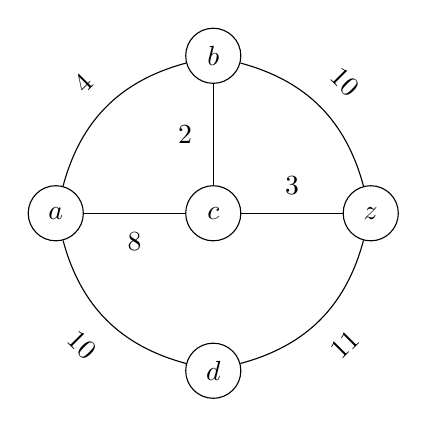
\begin{tikzpicture}[every node/.style={circle, draw, minimum size=0.7cm}]
                    % Nodes
                    \node (a) at (0, 0) {$a$};
                    \node (b) at (2,2) {$b$};
                    \node (c) at (2, 0) {$c$};
                    \node (d) at (2, -2) {$d$};
                    \node (z) at (4, 0) {$z$};
                
                    % Edges
                    % a to b
                    \draw (a) to [bend left=30] node [midway, above, sloped, outer sep=2pt, draw=none] {4} (b);
                    
                    % a to c
                    \draw (a) -- node [midway, below, draw=none] {8} (c);
                    
                    % a to d
                    \draw (a) to [bend right=30] node [midway, below, sloped, outer sep=2pt, draw=none] {10} (d);
    
                    % $b$ to c
                    \draw (b) -- (c) node [midway, left, draw=none] {2};
                    
                    % $b$ to z
                    \draw (b) to [bend left=30] node [midway, above, sloped, outer sep=2pt, draw=none] {10} (z);
                
                    % $c$ to z
                    \draw (c) -- (z) node [midway, above, sloped, draw=none] {3};
    
                    % $d$ to z
                    \draw (d) to [bend right=30] node [midway, below, sloped, outer sep=2pt, draw=none] {11} (z);
                
                \end{tikzpicture}
                \caption{Graph for Example 1}
            \end{figure}

        \begin{center}

        \begin{tabular}{c||c|c|c|c|c||l} 
        Step & $a$ & $b$ & $c$ & $d$ & $z$ & $S$\\

        \hline 
        $0$ & $\textcircled{0}$ & $\infty$ & $\infty$ & $\infty$ & $\infty$ & $\emptyset$\\
        $1$ & $\fbox{0}$ & $\textcircled{4}$ & $8$ & $10$ & $\infty$ & $\{a\}$\\
        $2$ & $\fbox{0}$ & $\fbox{4}$ & $\textcircled{6}$ & $10$ & $14$ & $\{a,b\}$\\
        $3$ & $\fbox{0}$ & $\fbox{4}$ & $\fbox{6}$ & $10$ & $\textcircled{9}$ & $\{a,b,c\}$\\
        $4$ & $\fbox{0}$ & $\fbox{4}$ & $\fbox{6}$ & $\textcircled{10}$ & $\fbox{9}$ & $\{a,b,c,z\}$\\
        
        \end{tabular}
        
        \end{center}

            \subsubsection{Walkthrough}
                \begin{enumerate}
                    \item We will start Step 0 by assigning our starting point a value of 0 and all other points a value of $\infty$. 0 is our smallest point value so it is circled.
                    
                    \item For Step 1, we move to our starting point and add it to our list $S$. A box is placed around point $a$'s value. It is adjacent to points $b$, $c$, and $d$ so we assign each adjacent point a value equal to the distance from our starting point. Point $b$ has the shortest distance, so it is circled.
                    
                    \item For Step 2, we move to point $b$ because it was the adjacent point with the shortest distance, and add it to our list $S$. A box is placed around point $b$'s value. We then look at the adjacent points, not in $S$, points $c$ and $z$. Calculate the distance value from each adjacent point to the current point plus the value of the current point, if it is lower than the adjacent point's current value, assign it the calculated value. Point $c$ has a calculated value of 6, which is less than its current value of 8, so it is assigned. Point $z$ has a calculated value of 14, which is less than its current value of $\infty$, so it is assigned. Point $c$ has the shortest distance so it is circled.
                    
                    \item For Step 3, we move to point $c$ because it was the adjacent point with the shortest distance, and add it to our list $S$. A box is placed around point $c$'s value. We look at the adjacent points not in $S$, point $z$. Calculate the distance value from the adjacent point to the current point plus the value of the current point, if it is lower than the adjacent point's current value, assign it the calculated value. Point $z$ has a calculated value of 9, which is less than its current value of 14, so it is assigned. Point $z$ has the shortest distance so it is circled.
                    
                    \item For step 4, we move to point $z$ because it was the adjacent point with the shortest distance, and add it to our list $S$. A box is placed around point $z$'s value. We look at the adjacent points not in $S$, point $d$. Calculate the distance value from the adjacent point to the current point plus the value of the current point, if it is lower than the adjacent point's current value, assign it the calculated value. Point $d$ has a calculated value of 20, which is not less than its current value of 10, so it is not assigned. Point $d$ has the shortest distance so it is circled. Since we've reached point $z$, we can halt our algorithm. Finally, we can extract $S$ as our shortest distance to point $z$.

                \end{enumerate}
        
        \subsubsection{Example 2}
            

            \begin{figure}[htbp]
                \centering
                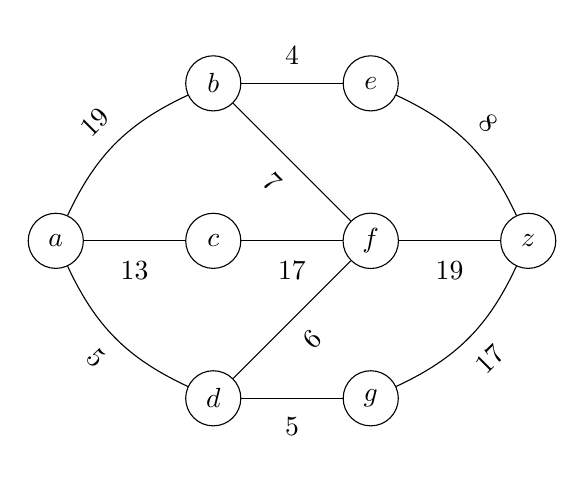
\begin{tikzpicture}[every node/.style={circle, draw, minimum size=0.7cm}]
                    % Nodes
                    \node (a) at (0, 0) {$a$};
                    \node (b) at (2, 2) {$b$};
                    \node (c) at (2, 0) {$c$};
                    \node (d) at (2, -2) {$d$};
                    \node (e) at (4, 2) {$e$};
                    \node (f) at (4, 0) {$f$};
                    \node (g) at (4, -2) {$g$};
                    \node (z) at (6, 0) {$z$};
                    
                
                    % Edges
                    % a to b
                    \draw (a) to [bend left=20] node [midway, above, sloped, draw=none] {19} (b);
                    
                    % a to c
                    \draw (a) -- node [midway, below, draw=none] {13} (c);
                    
                    % a to d
                    \draw (a) to [bend right=20] node [midway, below, sloped, draw=none] {5} (d);
    
                    % $b$ to f
                    \draw (b) -- (f) node [midway, below, sloped, draw=none] {7};
    
                    % $b$ to e
                    \draw (b) -- (e) node [midway, above, sloped, draw=none] {4};
                
                    % $c$ to f
                    \draw (c) -- (f) node [midway, below, sloped, draw=none] {17};
    
                    % $d$ to f
                    \draw (d) -- (f) node [midway, below, sloped, draw=none] {6};
    
                    % $d$ to g
                    \draw (d) -- (g) node [midway, below, sloped, draw=none] {5};
    
                    % $e$ to z
                    \draw (e) to [bend left=20] node [midway, above, sloped, draw=none] {8} (z);
                    
                    % $f$ to z
                    \draw (f) -- (z) node [midway, below, sloped, draw=none] {19};
    
                    % $g$ to z
                    \draw (g) to [bend right=20] node [midway, below, sloped, draw=none] {17} (z);
                
                \end{tikzpicture}
                \caption{Graph for Example 2}
            \end{figure}

            \begin{center}

            \begin{tabular}{c||c|c|c|c|c|c|c|c||l} 
            Step & $a$ & $b$ & $c$ & $d$ & $e$ & $f$ & $g$ & $z$ & $S$\\
            
            \hline
            $0$ & $\textcircled{0}$ & $\infty$ & $\infty$ & $\infty$ & $\infty$ & $\infty$ & $\infty$ & $\infty$ & $\emptyset$\\
            $1$ & $\fbox{0}$ & $19$ & $13$ & $\textcircled{5}$ & $\infty$ & $\infty$ & $\infty$ & $\infty$ & $\{a\}$\\
            $2$ & $\fbox{0}$ & $19$ & $13$ & $\fbox{5}$ & $\infty$ & $11$ & $\textcircled{10}$ & $\infty$ & $\{a,d\}$\\
            $3$ & $\fbox{0}$ & $19$ & $13$ & $\fbox{5}$ & $\infty$ & $11$ & $\fbox{10}$ & $\textcircled{27}$ & $\{a,d,g\}$\\
            $4$ & $\fbox{0}$ & $19$ & $13$ & $\fbox{5}$ & $35$ & $\textcircled{11}$ & $\fbox{10}$ & $\fbox{27}$ & $\{a,d,g,z\}$\\
            
            
            % Step 3 may not be needed.
            
            \end{tabular}
            
            \end{center}

                \subsubsection{Walkthrough}
                \begin{enumerate}
                    \item We will start Step 0 by assigning our starting point a value of 0 and all other points a value of $\infty$. 0 is our smallest point value so it is circled.
                    
                    \item For Step 1, we move to our starting point and add it to our list $S$. A box is placed around point $a$'s value. It is adjacent to points $b$, $c$, and $d$ so we assign each adjacent point a value equal to the distance from our starting point. Point $d$ has the shortest distance, so it is circled.
                    
                    \item For Step 2, we move to point $d$ because it was the adjacent point with the shortest distance, and add it to our list $S$. A box is placed around point $d$. We then look at the adjacent points, not in $S$, points $f$ and $g$. Calculate the distance value from each adjacent point to the current point plus the value of the current point, if it is lower than the adjacent point's current value, assign it the calculated value. Point $f$ has a calculated value of 11, which is less than its current value of $\infty$, so it is assigned. Point $g$ has a calculated value of 10, which is less than its current value of $\infty$, so it is assigned. Point $g$ has the shortest distance so it is circled.
                    
                    \item For Step 3, we move to point $g$ because it was the adjacent point with the shortest distance, and add it to our list $S$. A box is placed around point $g$. We look at the adjacent points not in $S$, point $z$. Calculate the distance value from the adjacent point to the current point plus the value of the current point, if it is lower than the adjacent point's current value, assign it the calculated value. Point $z$ has a calculated value of 28, which is less than its current value of $\infty$, so it is assigned. Point $z$ has the shortest distance so it is circled.
                   
                    \item For step 4, we move to point $z$,  because it was the adjacent point with the shortest distance, and add it to our list $S$. A box is placed around point z. We look at the adjacent points not in $S$, points $f$ and c. Calculate the distance value from the adjacent point to the current point plus the value of the current point, if it is lower than the adjacent point's current value, assign it the calculated value. Point $f$ has a calculated value of 36, which is not less than its current value of 11, so it is not assigned. Point $c$ has a calculated value of 35, which is less than its current value of $\infty$, so it is not assigned. Point $f$ has the shortest distance so it is circled. We will halt the algorithm because point $z$ has been reached. Finally, we can extract $S$ as our shortest distance to point $z$.
                \end{enumerate}



% ------------------------------------------------------------------------------
% Conclusion
% ------------------------------------------------------------------------------
    

\section{Conclusion}

    The world continually encounters the Shortest Path Problem, as discussed in our overview, exemplified by mapping applications like Google Maps. By illustrating Dijkstra's algorithm, we aim to present one of several solutions to this issue. Furthermore, we have successfully illustrated one of the pivotal aspects of Dijkstra's algorithm through our examples: time complexity. In Example 2, despite nearly doubling the potential points to visit, a solution was attained in the same number of steps. This crucial characteristic forms the basis for practical real-world applications, not solely theoretical ones. Additionally, we have devised an accessible method for coding a version of Dijkstra's algorithm by delineating the algorithm's steps in simple language and demonstrating how data might be stored by a computer using our tables.
        
\newpage

% ------------------------------------------------------------------------------
% End
% ------------------------------------------------------------------------------

\end{document}
